\section{Empirical analysis}
\label{sec:experiment}

\subsection{Datasets description}

\begin{figure*}[t]  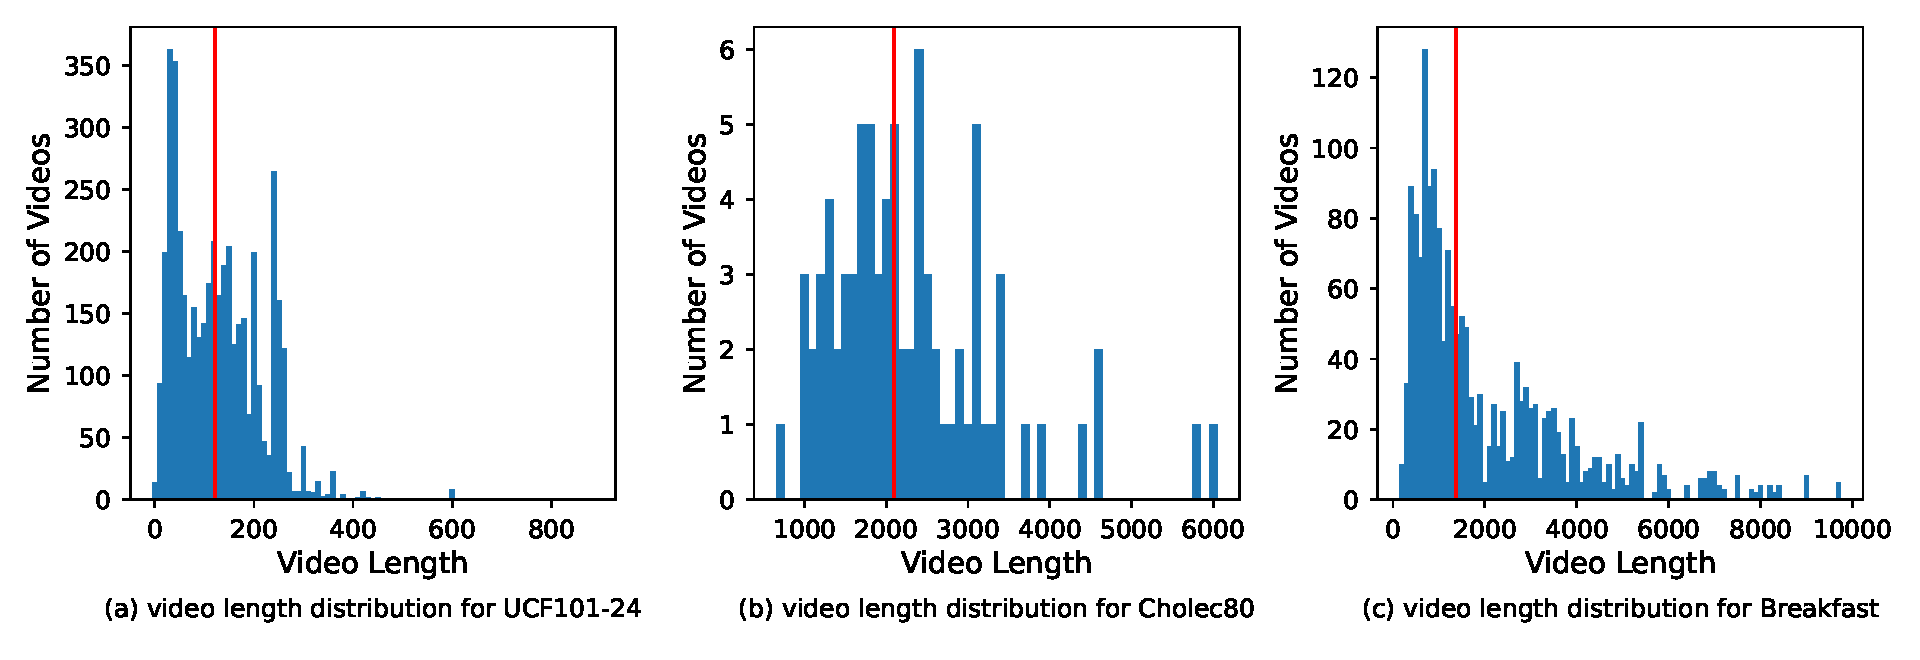
\includegraphics[width=1.0\linewidth]{iccv2023AuthorKit/media/dataset_lengths.pdf}
   \caption{Length distributions for \textsl{UCF101-24}, \textsl{Cholec80}, and \textsl{Breakfast}. \textsl{UCF101-24} are grouped into buckets of size 10, for \textsl{Cholec80} and \textsl{Breakfast} the buckets are of size 100. Most notable is the long tail length distribution on \textsl{Breakfast} which can make progress prediction more difficult.
   \slp{why do you use different bin sizes? Be consistent and use the same everywhere}}
\label{fig:lengths}
\end{figure*}

Each of the considered progress prediction methods evaluates on different datasets: \textsl{RSDNet} on \textsl{Cholec80} \cite{twinanda2016}, \textsl{ProgressNet} on \textsl{UCF101-24} \cite{soomro2012} and \textsl{UTE} on \textsl{Breakfast} \cite{kuehne2014, kuehne2016}. 
To analyze these methods we use all 3 datasets for all methods. 
Figure ~\ref{fig:lengths} shows the histogram of video lengths for each dataset. 
\textsl{Cholec80} has longer videos but the distribution is not very skewed \slp{I d not understand this, what distribution? skewed how?}. 
\textsl{UCF101-24} consists mainly of shorter videos \slp{So what if they are short? This says nothing. Conclude something}. 
Breakfast has quite a long tail of videos with many frames, which can make it extra challenging for progress prediction.
\slp{So is ucf simple? or cholec? You still dont conclude anything about the figure.}

\smallskip\noindent\textbf{\textsl{Cholec80} \cite{twinanda2016}}: Consists of 80 videos of endoscopic cholecystectomy surgery.  
Note that \cite{twinanda2019} uses an extended version of this dataset, \textsl{Cholec120}, containing 40 additional surgery videos. 
However, \textsl{Cholec120} is not publicly available, so we used \textsl{Cholec80} to report our results. 
We randomly create four folds of the data, and follow the same training\slash test dataset split sizes as \cite{twinanda2019}. 
This dataset has limited visual variability both across training and test splits.
Moreover, the presence of different medical tools in the frames informs of the different surgery phases, which could aid the progress prediction task.

% \slp{Add here what do you think? Is this an easy or a difficult task for progress prediction and why.}

\smallskip\noindent\textbf{\textsl{UCF101-24} \cite{soomro2012}:} Consists of a subset of \textsl{UCF101} containing 24 activities, each provided with a spatio-temporal action tube annotation \footnote{Following \cite{becattini2017} we use the revised annotations available at \url{https://github.com/gurkirt/corrected-UCF101-Annots}}. 
\cite{becattini2017} splits the dataset into 2 categories: \textsl{telic} and \textsl{atelic} activities. 
\textsl{Telic} activities are those with a clear end point, such as `cliff diving', while \textsl{atelic} activites, such as `walking', do not have a clearly defined end point. 
Predicting progress for \textsl{atelic} activities is more difficult than for \textsl{telic} ones.
The original implementation first trains on \textsl{telic} activities, and then fine-tunes on all activities. 
We did not observe a difference with this training procedure, and instead train all methods on the full dataset.

\smallskip\noindent\textbf{\textsl{Breakfast} \cite{kuehne2014, kuehne2016}:} Contains 10 cooking activities: \eg `making coffee', `baking pancakes', or `making tea', performed by 52 individuals in 18 different kitchens. 
We use the default splits and train each model across all cooking activities. 
Because the tasks are performed by different individuals in different kitchens, the video appearance varies even within the same task, making this dataset extra challenging for progress prediction.
% \slp{Add here what do you think? Is this an easy or a difficult task for progress prediction and why. Mention that you train one model across all cooking activities.}


\textsl{UCF101-24} contains videos of up to 599 frames, while \textsl{Cholec80} and \textsl{Breakfast} contain videos with thousands of frames.
When training on \textsl{full video} sequences we could not train the \textsl{ProgressNet} model on the full \textsl{Cholec80} and \textsl{Breakfast} datasets, because the model requires as input the complete video sequence as a sample.
Thus, for the experiments using \textsl{full videos} we use a subsampled version of \textsl{Cholec80} from 1 fps to 0.1 fps (the original fps is 25, \cite{twinanda2019} subsamples this down to 1fps); and we subsample \textsl{Breakfast} from 15 fps down to 1 fps. 
For our experiments on \textsl{video segments} we use the complete datasets.

% \begin{figure}[t]
% \begin{center}
%    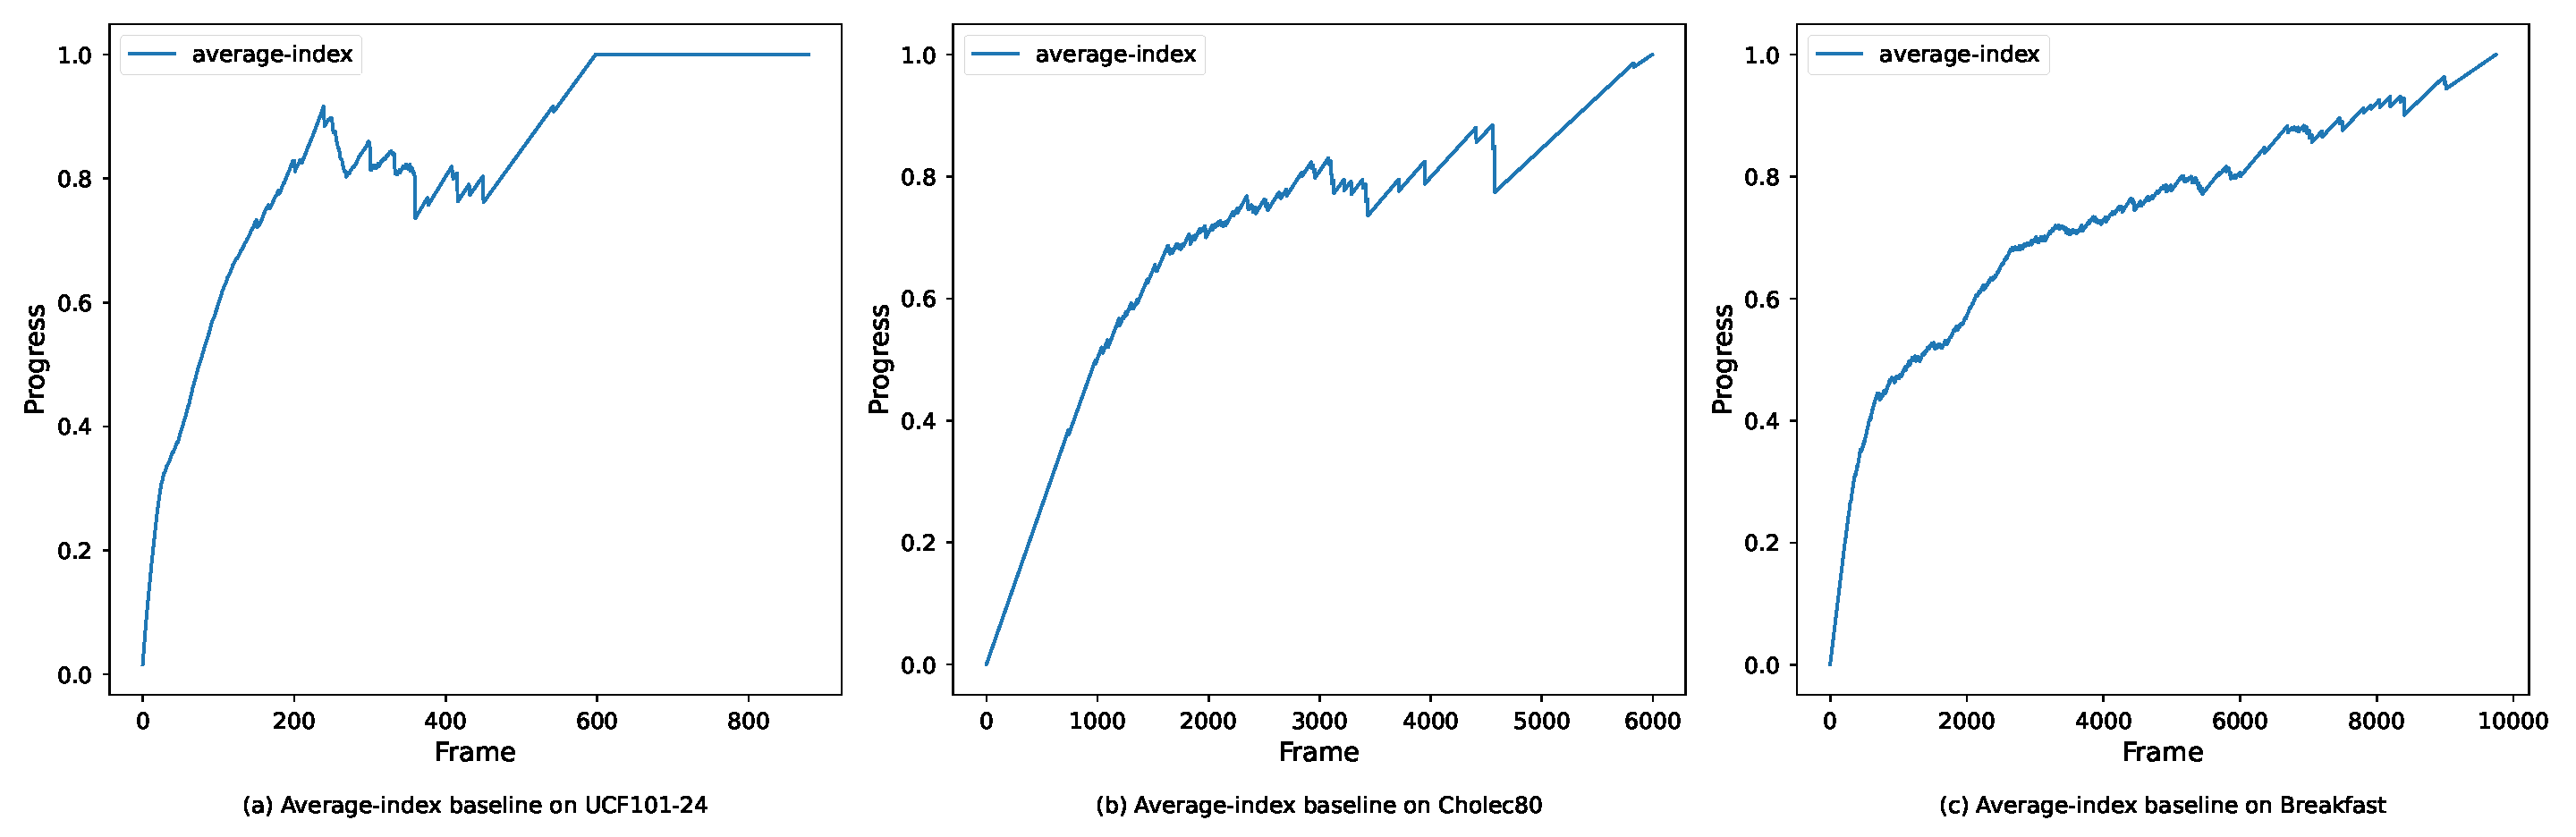
\includegraphics[width=1.0\linewidth]{iccv2023AuthorKit/media/avg_index_baseline.pdf}
% \end{center}
%    \caption{Average index baseline on Breakfast, UCF101-24, and Cholec80 
%    \slp{Why are you showing only the average index? What do you want people to see? 
%    Show all methods on a few examples if you want to show. Where is this referred in the text? Again use pdfs.}}
% \label{fig:averages}
% \end{figure}
%-----------------------------------------------------
\subsection{Experimental setup}
%\frans{TODO: Move network descriptions from here to section 3.1, change this to training setup}

Of the considered methods only the code for \textsl{UTE} is published.\footnote{\url{https://github.com/Annusha/unsup_temp_embed}} 
For the other methods we follow the papers for implementation details and training procedures. 
We train \textsl{RSDNet} in a 2-step procedure following \slp{cite \cite{}}, however for the training of the LSTM blocks we found that using the Adam optimizer with a learning rate of $10^{-4}$ and no weight decay, for $30$k iterations works best. 
For \textsl{ProgressNet} \slp{cite \cite{} does not provide the training details}, so we use Adam with a learning rate of $10^{-4}$ for $50$k iterations, and we keep the VGG-16 backbone frozen during training. 
For all experiments we report the MAE (Mean Absolute Error) in percentages.

% ------ Old ----------
% We strive to follow the original papers implementation as close as possible. For \textsl{UTE} the code is published  online\footnote{\url{https://github.com/Annusha/unsup_temp_embed}} so we use this. For \textsl{RSDNet} and \textsl{ProgressNet} no code is available so we implement these ourselves.

% For \textsl{RSDNet} we implement the model following the procedure from the paper \cite{twinanda2019} and train it in a two-step way. First, we take a ResNet152 model pretrained on Imagenet and train it to predict progress from independent $2D$ images. After this, we use the trained ResNet152 network to create embeddings for all frames and input this to the LSTM layer of \textsl{RSDNet}. These same embeddings are used to train the \textsl{ResNet-LSTM}. For both networks the LSTMs have 512 hidden nodes.

% We also implement \textsl{ProgressNet} from scratch. For the backbone we use a VGG-16 model pretrained on ImageNet. We use SPP layers of sizes $1$, $2$, and $3$ and a ROI pooling of size $3$. The two linear layers \textsl{fc6} each have 1024 nodes and the outputs are concatenated. The two LSTMS have 64 and 32 hidden nodes.
\subsection{\textbf{\emph{(i) On what information do progress prediction methods base their predictions?}}}
\noindent\textbf{(i.1) Progress predictions on full videos.}
For our first experiment we consider training the methods on full video sequences as is done in \cite{twinanda2019} \slp{Why do we consider this? Motivate what is the purpose of this experiment? What do you expect it to show? Why do you compare with random? e.g. 
"Here we want to test what information are the learning-based models using when trained on full videos to predict activity progress.
For this we ..."
}. 
We compare giving \slp{inputting into} the methods the full video data: \ie either frames or frame embeddings, or \textsl{random noise}. We expect that in both cases the methods may learn how to count and will approximate the \textsl{Average Index} baseline. The results can bee seen in figures ~\ref{fig:result_ucf_seq}, ~\ref{fig:result_breakfast_seq} and \ref{fig:result_cholec_seq}.
\slp{Rewrite the above sentence as:
For the the learning-based methods (\textsl{..}, ..) we evaluate their MAE scores when they receive as input the \textsl{full video} data compared to \textsl{random} noise. 
Additionally we report the MAE scores for the non-learning baselines: \textsl{...}
}

% \slp{Say here what is the setting, what do you compare with what and why and what is the expected finding.}


% \frans{Still need to explicitly mention the expectation that a "counting network" will perform on par with the average index baseline}

\begin{figure}
\begin{center}
   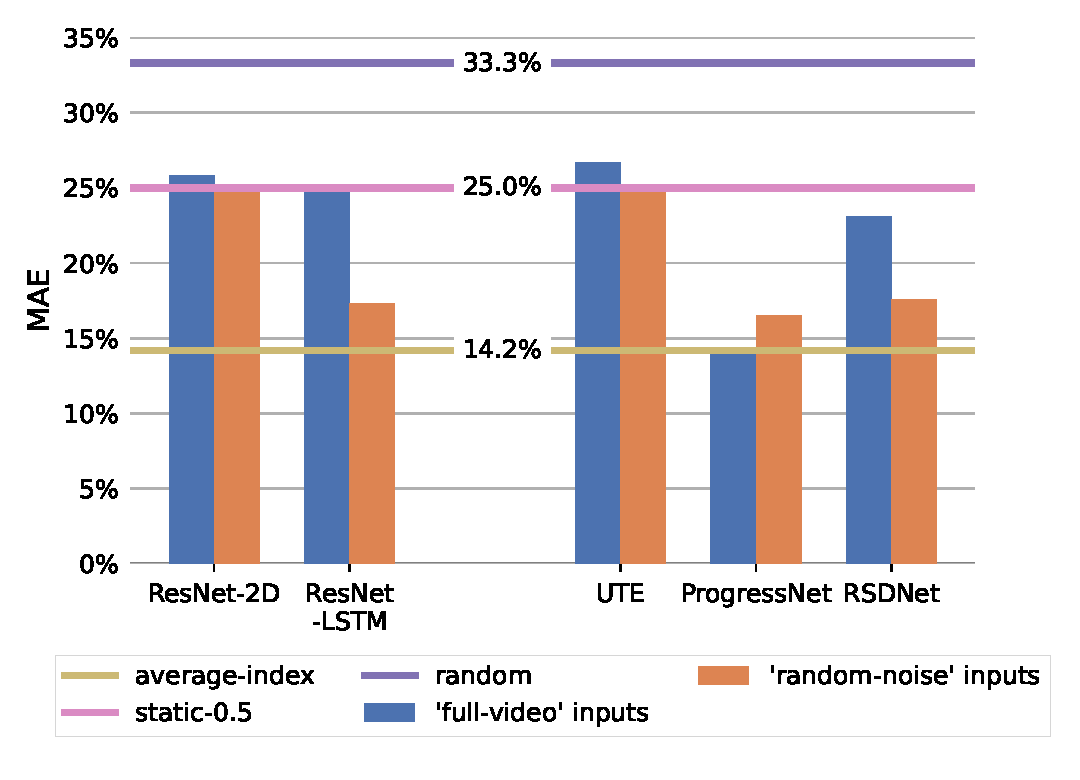
\includegraphics[width=1.0\linewidth]{iccv2023AuthorKit/media/results/UCF101-24_full_video_random.pdf}
\end{center}
   \caption{\textbf{UCF101-24 training on \textsl{full videos}}. MAE in percentages for all considered methods on when inputting both video frames and random noise. For all methods except \textsl{ProgressNet} inputting random noise to the LSTM based methods performs on par or better than when inputting video frames.
   \slp{Please clarify in all captions that "full videos" are input and "random noise" as well: e.g. "`full video' inputs". Now you have 2 random and that is confusing because one is a baseline and the other is an input. Also use "static-0.5".
   Also not that I use "textsl" for all dataset names and method names and data settings.}
   }
\label{fig:result_ucf_seq}
\end{figure}
\begin{figure}
\begin{center}
   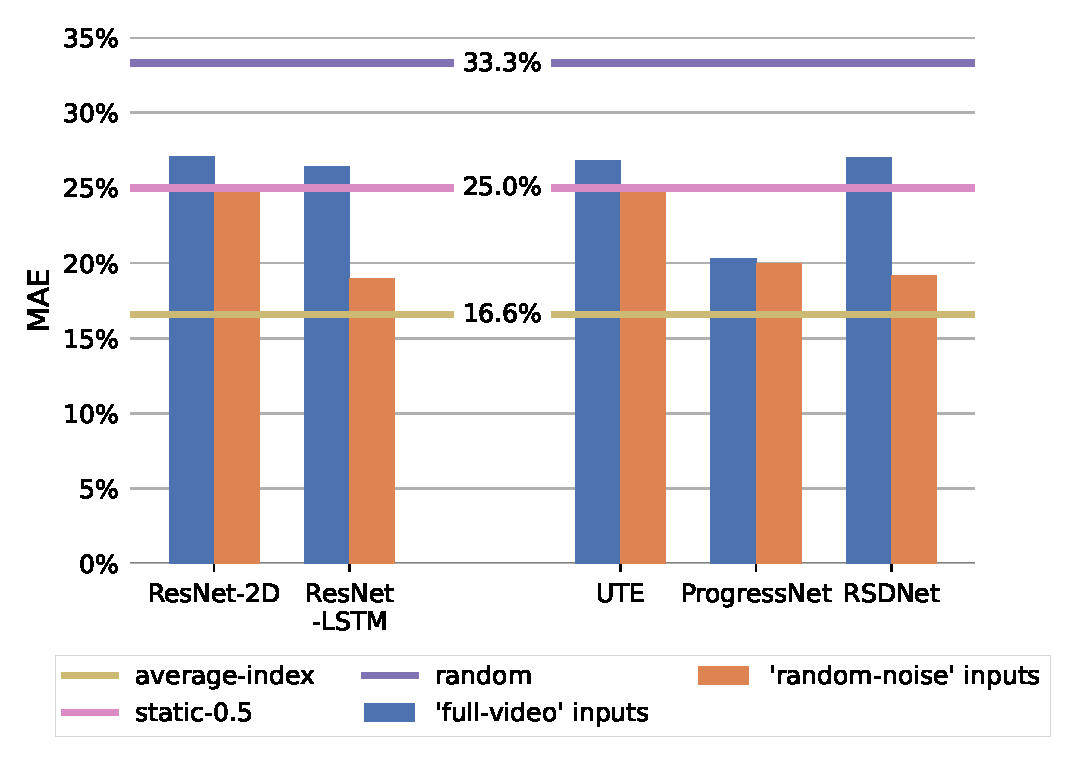
\includegraphics[width=1.0\linewidth]{iccv2023AuthorKit/media/results/Breakfast_full_video_random.pdf}
\end{center}
   \caption{\textbf{Breakfast training on \textsl{full videos}}. 
   MAE in percentages for all considered methods on when inputting both video frames and random noise. For all methods inputting random noise to the LSTM based methods performs on par or better than when inputting video frames.}
\label{fig:result_breakfast_seq}
\end{figure}
\begin{figure}
\begin{center}
   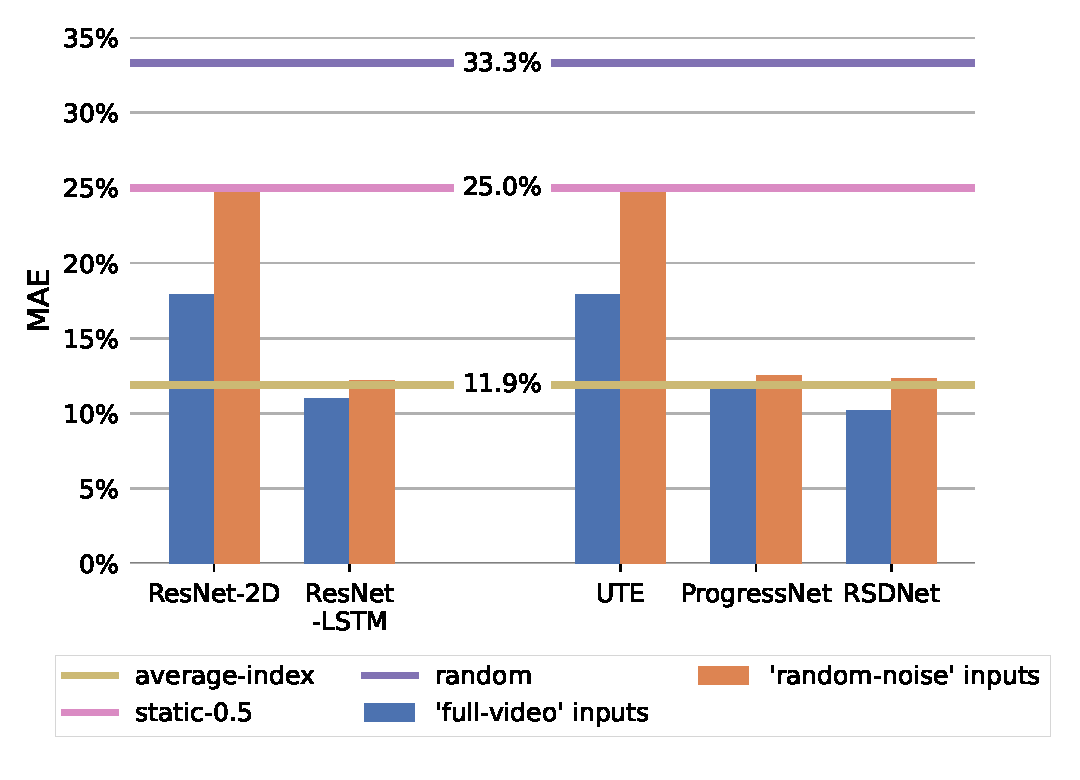
\includegraphics[width=1.0\linewidth]{iccv2023AuthorKit/media/results/Cholec80_full_video_random.pdf}
\end{center}
   \caption{\textbf{Cholec80 training on \textsl{full videos}}. 
   MAE in percentages for all considered methods on when inputting both video frames and random noise. All methods are able to learn from real video data. When given random noise the LSTM based methods perform on par with the \textsl{Average Index} baseline.}
\label{fig:result_cholec_seq}
\end{figure}

\slp{For consistency use the macros: \fig, \eq, \tab to refer to figures/equations/tables everywhere.}

\fig{result_ucf_seq} shows that when training on \textsl{full videos} of \textsl{UCF101-24} both the \textsl{ResNet152-2D} model and \textsl{UTE} models perform on par with the \textsl{static-0.5} baseline.
This is because these spatial-only networks do not have any way of integrating temporal information and they fail to extract progress information from the visual data alone. 
When provided with \textsl{random} noise they always predict 0.5 and score on par with the \textsl{static-0.5} baseline. 
The results are similar for the recurrent models, \textsl{ResNet152-LSTM} and \textsl{RSDNet}: they are both close to the \textsl{static-0.5} baseline. 
This is because the networks overfit on the embedded features and do not generalise to the test set. When these recurrent networks are provided with random noise they learn to count frames, and thus reach the \textsl{average index} baseline. 
\textsl{ProgressNet} is the only outlier here: when given \textsl{full video} data it performs better than the \textsl{average index} baseline, and when given \textsl{random} data it performs slightly worse. 
Since the visual information is not sufficiently informative to predict progress, \textsl{ProgressNet} learns to count frames to aid in its progress predictions.

For Breakfast in Figure ~\ref{fig:result_breakfast_seq} the results look very similar. Both the \textsl{ResNet152-2D} and \textsl{UTE} models cannot learn from visual information alone. ResNet152-LSTM and RSDNet both perform worse than the Static 0.5 baseline, indicating that they are overfitting on the training data. When given random noise they start counting frames again. ProgressNet gets similar results when given both real video data and random noise, indicating that in both cases it is doing frame counting.

Cholec80 in Figure ~\ref{fig:result_cholec_seq} is the first dataset where the spatial only networks \textsl{ResNet152-2D} and \textsl{UTE} perform better than the Static 0.5 baseline, indicating that there is visual information in this dataset the networks can learn. When given random noise they again perform on par with the Static 0.5 baseline. ResNet152-LSTM, RSDNet, and ProgressNet, can make use of the visual information and frame counting and perform slightly better than the \textsl{Average Index} baseline. These networks perform slightly worse, but still on par with the \textsl{Average Index} baseline when given random data.

\noindent\textbf{Observation:} \emph{We conclude that the progress prediction methods and the learning baselines may fail to make effective use of the visual data present in the videos. Instead they either overfit on the training data, or rely on simple frame counting.}

%-----------------------------------------------------------------------------------
\medskip\noindent\textbf{(i.2): Progress predictions on video segments.}
For our second experiment we consider training the methods on video segments as is done in \cite{becattini2017}. We compare giving the methods \textsl{real video data}, either frames or frame embeddings, and \textsl{frame indices}. To predict the progress $p_{i}$ for frame $i$ we give the methods the value $i$ divided by the average length of a sequence in the dataset. We expect that when given \textsl{real video data} the methods perform worse than in Experiment 1 because they can no longer count, and when given \textsl{frame indices} they start approaching the \textsl{Average Index} baseline. The results can be seen in Figures ~\ref{fig:result_ucf_seg}, ~\ref{fig:result_breakfast_seg} and ~\ref{fig:result_cholec_seg}.
% \slp{Say here what is the stting, what do you compare with what and why and what is the expected finding.}

\begin{figure}
\begin{center}
   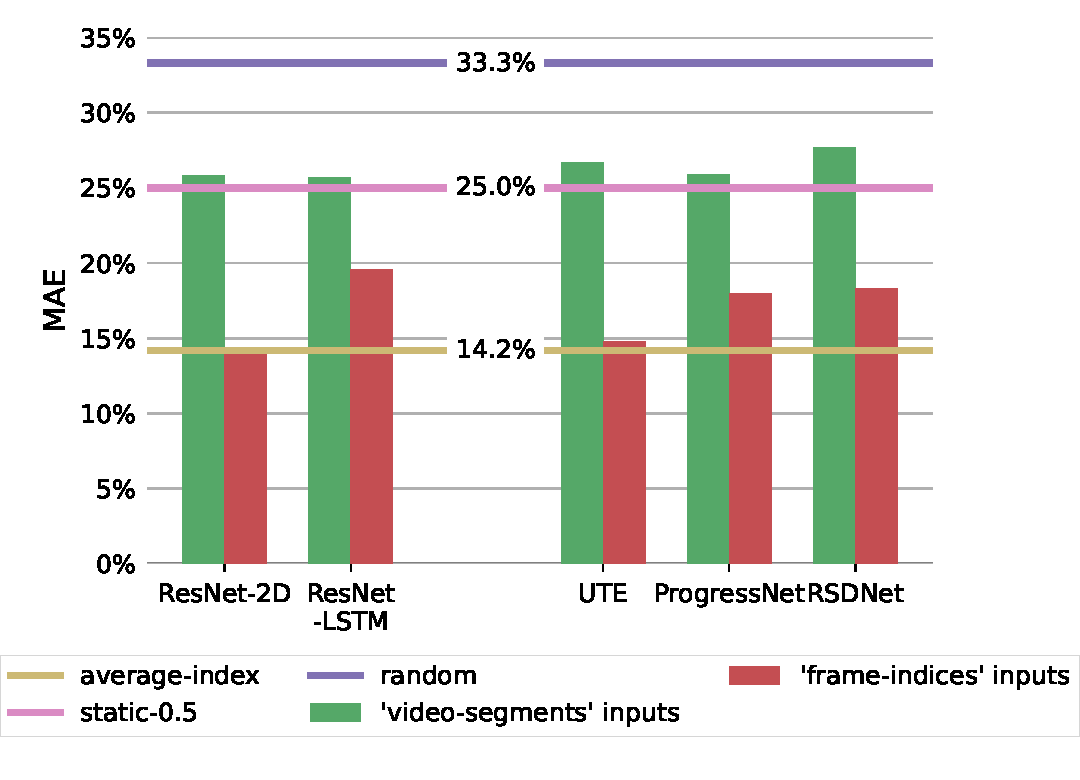
\includegraphics[width=1.0\linewidth]{iccv2023AuthorKit/media/results/UCF101-24_video_segments_indices.pdf}
\end{center}
   \caption{\textbf{UCF101-24 training on \textsl{video segments}}. MAE in percentages for all considered methods on when inputting both video frames and frame indices. For all methods inputting frame indices to the model performs better than when inputting video frames. ResNet152 and UTE get the biggest boost in performance.}
\label{fig:result_ucf_seg}
\end{figure}
\begin{figure}
\begin{center}
   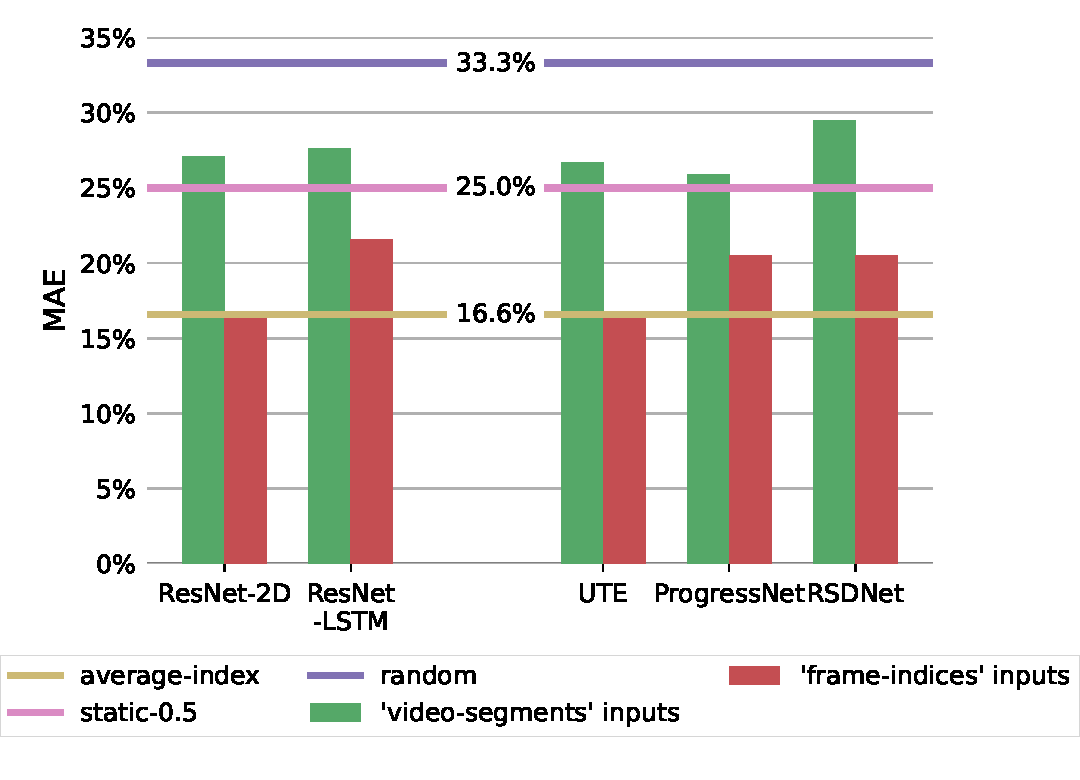
\includegraphics[width=1.0\linewidth]{iccv2023AuthorKit/media/results/Breakfast_video_segments_indices.pdf}
\end{center}
   \caption{\textbf{Breakfast training on \textsl{video segments}}. MAE in percentages for all considered methods on when inputting both video frames and frame indices. For all methods except RSDNet inputting frame indices to the model performs better than when inputting video frames. ResNet152 and UTE get the biggest boost in performance.}
\label{fig:result_breakfast_seg}
\end{figure}
\begin{figure}
\begin{center}
   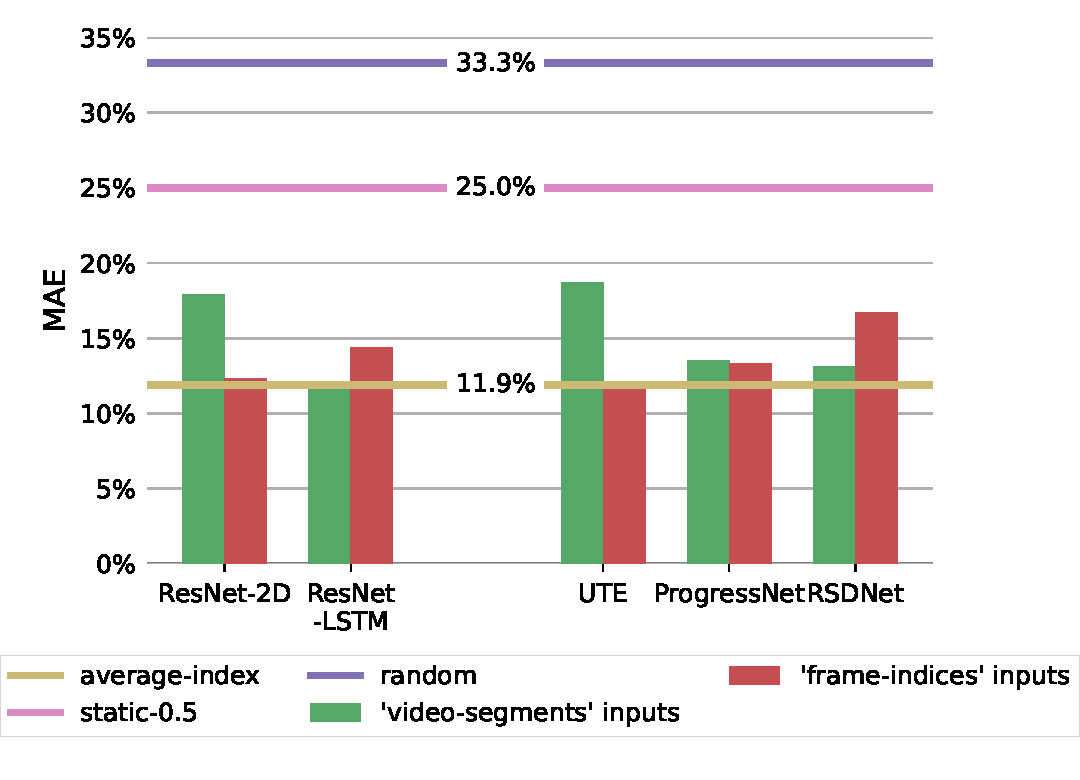
\includegraphics[width=1.0\linewidth]{iccv2023AuthorKit/media/results/Cholec80_video_segments_indices.pdf}
\end{center}
   \caption{\textbf{Cholec80 training on \textsl{video segments}}. MAE in percentages for all considered methods on when inputting both video frames and frame indices. For all methods except RSDNet inputting frame indices to the model performs better than when inputting video frames. ResNet152 and UTE get the biggest boost in performance.}
\label{fig:result_cholec_seg}
\end{figure}

   % \caption{\textbf{Cholec80 training on \textsl{full videos}}. 
   % MAE in percentages for all considered methods on when inputting both video frames and random noise. All methods are able to learn from real video data. When given random noise the methods perform on par with the \textsl{Average Index} baseline.}
The first thing we can observe on UCF in Figure ~\ref{fig:result_ucf_seg} is that when given video segments all methods perform on par with the Static 0.5 baseline, meaning that they cannot learn anything from the data. This is especially interesting for ProgressNet, which on full sequences in Figure ~\ref{fig:result_ucf_seq} was able to improve over the \textsl{Average Index} baseline. This result indicates that before the network was not learning from the visual information, but just like when given random noise it was learning to count. When given indices all methods improve. This improvement is the most significant for ResNet152 and UTE, which almost exactly match the average index baseline. might not be able to exactly match the average index baseline because of the length of the sequences.

The results on Breakfast in Figure ~\ref{fig:result_breakfast_seg} are again very similar to those of UCF. None of the networks are able to learn anything from the real data, and ProgressNet now performs worse than when it is trained on full sequences. All methods except for RSDNet see an improvement when trained on indices, and this improvement is the most significant for ResNet152 and UTE. RSDNet appears to perform worse on the progress prediction, we hypothesise that this is due to the joint optimization of both progress and RSD.

For Cholec80 in Figure ~\ref{fig:result_cholec_seg} we see that most methods perform very similar. ResNet-2D and UTE see an improvement when given indices, but for ResNet-LSTM and ProgressNet the performance is on par with the \textsl{Average Index} baseline when given both real video data and indices. This result indicates that on the Cholec80 dataset the methods are able to learn from visual information, however they still cannot perform better than the \textsl{Average Index} baseline.

\smallskip\noindent\textbf{Observation:} \emph{We conclude that the progress prediction methods cannot perform well on video segments because the visual data does not contain sufficient information for solving the progress prediction task and the networks can no longer rely on simple frame counting.}


%-------------------------------------------------------------------------------
\subsection{\emph{\textbf{(ii) Is it feasible to predict activity progression form visual data only?}}}
We observe that existing learning-based methods often fail to extract progress information form visual data alone. Our goal here is to construct a synthetic dataset in such a way that the learning-based methods perform optimally using visual information, and the naive baselines perform worse.

We construct a synthetic dataset containing progress bars, as shown in Figure ~\ref{fig:progressbars}. The dataset videos contain progress bar (similar, for example, to a download bar) that slowly fills up from left to right. Each bar has its own rate of progression, but there is a variance per notch causing some uncertainty. This is why for example the first image visually looks to be slightly beyond 25\%, but because the video may slow down after this section it is actually at 22.2\%. Because of the different progress rates per video, and the variance in progress rate in a video, the learning methods cannot just rely on visual information alone but will also have to use memory to perform well on the progress prediction task. Moreover, due to the large variance in video length the \textsl{Average Index} baseline, and thus counting, will perform worse than using visual information.


% \slp{Say here what is the stting, what do you compare with what and why and what is the expected finding.}


\begin{figure}[t]
\begin{center}
   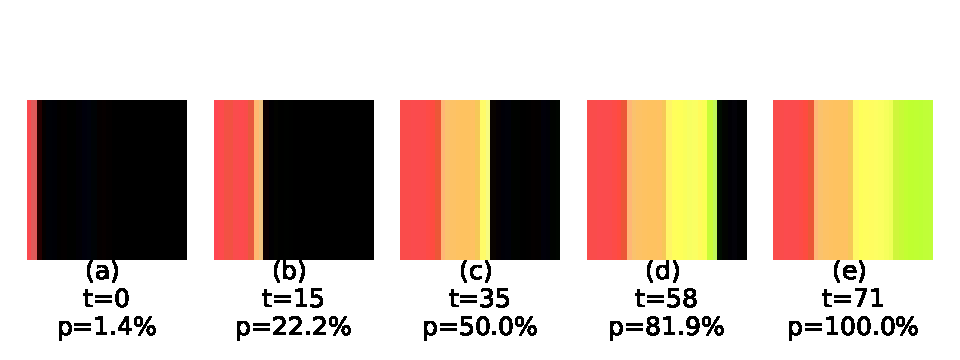
\includegraphics[width=1.0\linewidth]{iccv2023AuthorKit/media/bars.pdf}
\end{center}
   \caption{Visualisation of 1 progress bar from the syntethic dataset at timesteps $t=0$, $t=15$, $t=35$, $t=58$, and $t=71$. Each coloured section indicates visually a 25\% section, but due to variance in the speed the actual progress may differ at these points.
   % \slp{Can you change the color scheme into something more pleasing for the eyes. Also I cannot read the text. Also make it pdf. You can export all figures from python as pdfs. If you need to edit them use inkscape.}
   % \slp{Say something about this: what are the colors, what is each row, each column? What is the conclusion? What should we see in the figure?}
   % \slp{It is unclear that these are video frames, can you add labels on top}
   }
\label{fig:progressbars}
\end{figure}

Figure ~\ref{fig:result_bars} shows the results of the considered progress prediction methods, the learning-based baselines and the naive baselines on both sequences and segments. For this dataset the \textsl{Average Index} baseline gets an \textbf{MAE} of 12.9, which gets outperformed by all learning-based methods. We see that UTE performs the best out of all networks even though it does not have memory. This is because UTE is trained on frame embeddings with a window size of 15. This window gives the method information about 7 future frames, which gives it a significant advantage on such a simple dataset. With the LSTM based methods we see that giving full video sequences performs slightly better than giving video segments.

\smallskip\noindent\textbf{Observation:} \emph{We conclude that the progress prediction methods can make effective use of the visual data present in the videos and outperform the \textsl{Average Index} baseline.
}
\begin{figure}
\begin{center}
   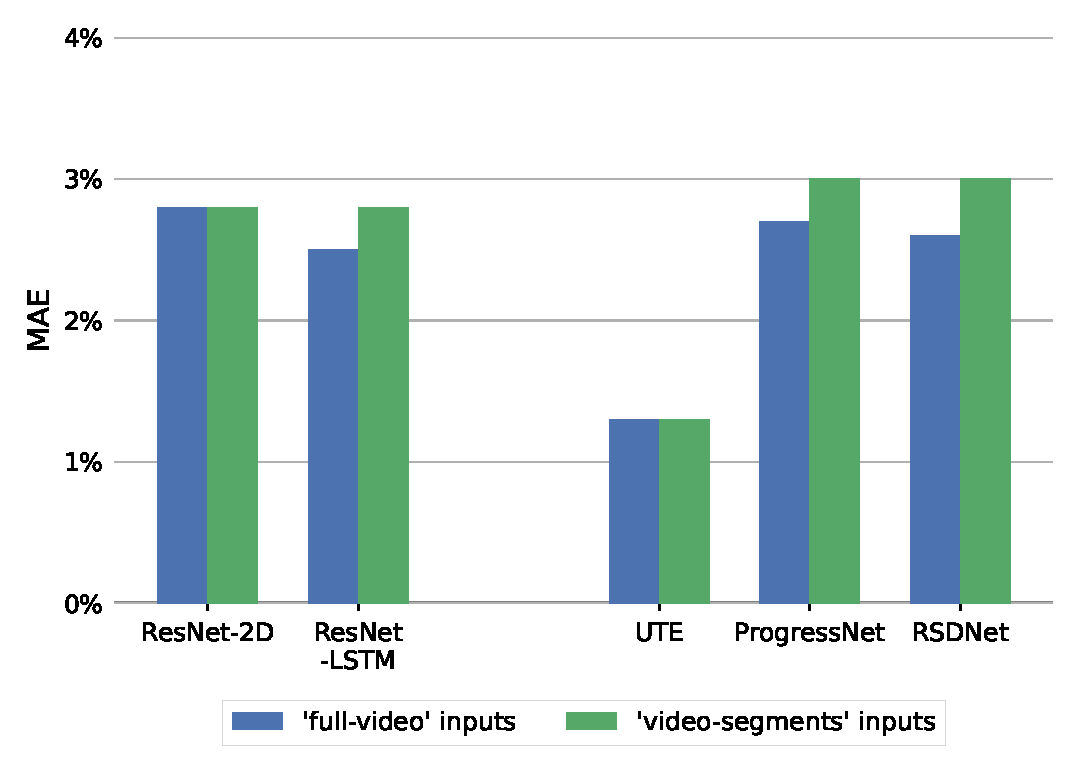
\includegraphics[width=1.0\linewidth]{iccv2023AuthorKit/media/results/Bars_full_video_video_segments.pdf}
\end{center}
   \caption{\textbf{Syntethic progress bars datset training on \textsl{full videos} and \textsl{video segments}}. MAE in percentages for all considered methods on when inputting both video frames and frame indices. \textsl{Average Index} is $12.9\%$. We see that all methods outperform the \textsl{Average Index} baseline. \textsl{UTE} gets the best result due to its 15 frame temporal window allowing it to see 7 frames into the future which gives a significant advantage on such a simple dataset. From this we can conclude that the progress prediction methods are able to learn progress from visual information if it is clearly present in the videos.}
\label{fig:result_bars}
\end{figure}